\subsubsection{Minuta de reunião (12-Agosto-2015)}

\begin{tabbing}
  Local \= xxx \kill
  Local \> : LEAD \\
  Data  \> : 12 de Agosto de 2015 \\
  Hora  \> : 13:00
\end{tabbing}

%---------------------------------------------------------------------
\participantes{
  \elael,
  \alana,
  \gabriel,
  \julia,
  \estevão,
  \renan.
}

\textbf{Aprovação da minuta}

\textbf{Update semanal do Projeto EMMA}
   							
\textbf{\elael.} 
	\begin{itemize}
		\item \textbf{Tarefas concluídas:}
			\begin{itemize}    
				\item Pesquisa de sensores de point laser. 
			\end{itemize}
		
		\item \textbf{Novas tarefas:}
			\begin{itemize} 
				\item: Escolher equipamento para calibração.
				\item: Começar mexer com o LMS111 Laser scan. 
			\end{itemize}
	\end{itemize}
	
	\textbf{\Julia.} 
	\begin{itemize}
		\item \textbf{Tarefas concluídas:}
			\begin{itemize}    
				\item ADM: Passagens e viagem CITENEL
				\item Acerto de possível co-orientadora para mestrado, ajustes na proposta
				de acordo.
			\end{itemize}
		
		\item \textbf{Novas tarefas:}
			\begin{itemize} 
				\item: Apresentação de Metodologia para o design de interface do software do
				projeto.
			\end{itemize}
	\end{itemize}
					
\textbf{\gabriel.} 
	\begin{itemize}
		\item \textbf{Tarefas concluídas:}
			\begin{itemize}    
				\item Pesquisa de Sensores 2D.
			\end{itemize}
		
		\item \textbf{Novas tarefas:}
			\begin{itemize} 
				\item Escolher equipamento para calibração.
				\item Começar mexer com o LMS111 Laser scan. 
				\item Reuniões com diferentes fornecedores de sensores. (NIKON, FARO,
				LEICA, CIK).
			\end{itemize}
	\end{itemize}
					
			
   \textbf{\estevão.} 
	\begin{itemize}
		\item \textbf{Tarefas concluídas:}
			\begin{itemize}    
				\item Apresentação sobre Cinemática dos braços robóticos possíveis, 
				tabela comparativa, pontos fortes e fracos.
				\item Estudo de diferentes supporte para a solução da escotilha inferior,
				desenhos de solid works.
			\end{itemize}
		
		\item \textbf{Novas tarefas:}
			\begin{itemize} 
			    \item Desenho Motoman sem graus de liberdade.
			    \item Maquete: Possibilidades de execução junto a EBA e justificativa
			    técnica para rúbrica de serviços.
			\end{itemize}
	\end{itemize}

			
   \textbf{\Renan.} 
	\begin{itemize}
		\item \textbf{Tarefas concluídas:}
			\begin{itemize}    
				\item Apresentação sobre Cinemática dos braços robóticos possíveis, 
				tabela comparativa, pontos fortes e fracos.
				\item Estudo de diferentes supporte para a solução da escotilha inferior,
				calculos e comparação de áreas de coating possíveis.
			\end{itemize}
		
		\item \textbf{Novas tarefas:}
			\begin{itemize} 
			    \item Checar os alcance dos braços escolhidos em 30 graus.
			\end{itemize}
	\end{itemize}		



\textbf{Agenda para a próxima reunião:}
  \begin{itemize}
    \item Resultado de pesquisas individuais.
    \item Novas tarefas \& recomendações.
  \end{itemize}


\vspace{5mm}%
\parbox[t]{70mm}{
  Aprovado por: \\[5mm]
  \centering
  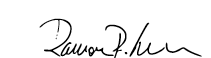
\includegraphics[width=65mm]{figs/logo/assinatura-ramon.png} \\[-4mm]
  \rule[2mm]{70mm}{0.1mm} \\
  \ramon \\[1mm]
  Coordenador do Projeto \\
}

%---------------------------------------------------------------------
\fim